This use-case is the implementation of an \emph{hybrid} use-case that embodies
both the automatic and the human scenario. In the matrix at \autoref{tab:matrix}
this use case is placed between the human and the automatic, voluntary, scenario.

\begin{figure}[htb]
    \centering
    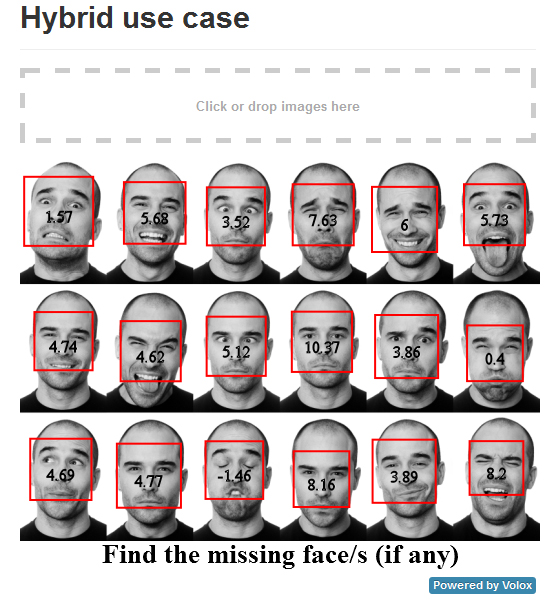
\includegraphics[width=0.75\columnwidth]{Hybrid}
    \caption{Interface of the hybrid use-case.}
    \label{fig:Hybrid1}
\end{figure}

This use-case has the purspose of \emph{detecting faces} in a picture, to
accomplish this task are used an automatic face recognition algorithm\footnote{
Available at \url{https://github.com/liuliu/ccv/tree/unstable/js} with a demo
application here: \url{http://liuliu.me/ccv/js/nss/}} plus a human interacition
that has the double purpose of validating the algotithm result and detect the
missing faces in the image.\\

This scenario is implemented in 2 steps, in the first step we run the algorithm
for detecting the faces (this is the \emph{automatic} scenario), in the second
step we present a subset of detected faces to the user asking to find the
missing faces. We need to remove some result from the set in order to check the
trustworthiness of the user.\\

At the end of the execution we obtain a set of automatically detected faces plus
all the faces detected by the user. By intersecting this two set we could improve
the performance of our algorithm by adding the faces it was unable to find to
the training set.

\subsubsection{Benchmark/Metric}
With this hybrid approach we are able to stress all the matrix in with a single
example. The most similar approach to this solution is \ac{GWAP}.

TODO ???